\documentclass[11pt]{article}
\usepackage[a4paper,margin=1in]{geometry}
\usepackage{amsmath,amssymb,amsfonts,amsthm}
\usepackage{booktabs}
\usepackage{graphicx}
\usepackage{hyperref}
\usepackage{microtype}
\usepackage{enumitem}
\usepackage{array}
\usepackage{caption}
\usepackage{subcaption}
\usepackage{xcolor}
\hypersetup{colorlinks=true,linkcolor=blue,citecolor=blue,urlcolor=blue}
\graphicspath{{paper_assets/}}

\newcommand{\Cl}{\mathrm{Cl}}
\newcommand{\C}{\mathbb{C}}
\newcommand{\Tr}{\mathrm{Tr}}
\newcommand{\ii}{\mathrm{i}}
\newcommand{\ket}[1]{\left|#1\right\rangle}
\newcommand{\bra}[1]{\left\langle#1\right|}
\newcommand{\expval}[1]{\left\langle #1 \right\rangle}
\newcommand{\norm}[1]{\left\lVert #1 \right\rVert}

\newtheorem{proposition}{Proposition}
\newtheorem{lemma}{Lemma}
\newtheorem{corollary}{Corollary}
\newtheorem{remark}{Remark}

\title{Operator-Centric Variational Quantum Eigensolvers\\ in Clifford Algebra}

\author{
Ginanjar Utama\\[-2pt]
\normalsize\texttt{ginanjar.utama@gmail.com}
\and
Hermawan K.\ Dipojono\\[-2pt]
\normalsize\texttt{dipojono@itb.ac.id}
}
\date{}

\begin{document}
\maketitle
\begin{center}
\vspace{-1.5em}
\normalsize Institut Teknologi Bandung, Indonesia\\[2pt]
\normalsize July 2026
\end{center}

\begin{abstract}
We formulate variational quantum eigensolvers entirely inside the complex Clifford algebra $\Cl(2n,\C)\cong M(2^n,\C)$, in an operator-centric picture in which states, gates, observables, quantum channels, fermionic modes, and even the operator-selection gradients of adaptive methods are elements of one algebra.  Density operators are multivectors evolved by two-sided sandwiches, expectation values are scalar parts of geometric products, and the Jordan--Wigner transformation is an internal change of basis rather than an external translation step.  On this foundation we study the one-dimensional transverse-field Ising model with two variational methods: a fixed-depth Hamiltonian variational ansatz built from Pauli-word rotations $\exp(-\ii\theta P/2)$, and an ADAPT-VQE scheme whose selection scores $\Tr(\rho\,[H,P])$ are Hermitian commutator observables estimated from finite-shot measurements with cumulative shot escalation and heuristic rank-resolution gates.  A reality selection rule, proved in the operator-centric language, shows that only Pauli words with an odd number of $Y$ factors can carry a nonzero selection gradient for real Hamiltonians and real states, fixing the operator pool a priori.  For the four-site critical open chain, the depth-three ansatz reaches relative energy error $4.8\times10^{-5}$ with fidelity $0.99995$; exact ADAPT reaches numerical ground-state accuracy with six operators; and finite-shot ADAPT remains variational and monotone, trading measurement cost against ranking reliability.  We claim no asymptotic speedup: the contribution is a compact algebraic formulation in which Pauli-rotation calculus, Clifford sparsity, measurement statistics, and adaptive ansatz growth are expressed in a single computational language.
\end{abstract}

\section{Introduction}

Variational quantum algorithms were proposed as hybrid methods suitable for near-term processors, with the variational quantum eigensolver (VQE) using a parameterized quantum circuit and a classical optimizer to minimize an energy expectation value \cite{peruzzo2014vqe}.  A central practical difficulty is ansatz design: fixed hardware-efficient circuits may be shallow but poorly matched to the problem, while chemically or physically motivated ansatzes may be deeper.  ADAPT-VQE addresses this by growing the circuit one operator at a time, choosing the next operator from a pool by a gradient criterion \cite{grimsley2019adapt}; qubit-ADAPT variants further emphasize hardware-efficient operator pools \cite{tang2021qubitadapt}.  In realistic settings, however, the operator-ranking gradients themselves are estimated from finite measurements.  An adaptive algorithm can therefore fail before the optimization begins: the wrong operator may be selected because the ranking signal is statistical.

This paper studies these questions in a single algebraic language.  Rather than treating state vectors, matrices, Pauli strings, channels, and fermionic modes as separate mathematical objects, we represent every object as an element of one algebra,
\begin{equation}
    \Cl(2n,\C) \cong M(2^n,\C),
\end{equation}
in the \emph{operator-centric} picture.  Clifford-algebraic qubit constructions have most often been developed in a spinor / minimal-left-ideal form \cite{hrdina2022clifford}; the explicitly operator-centric density-multivector proposal used here, in which the state is the density operator itself rather than an ideal element, follows Silva \cite{silva2025operator}, within the broader tradition of geometric-algebra reformulations of quantum mechanics \cite{hestenes2003oersted}.  Section~\ref{sec:operator-centric} develops this picture in detail: it is not a notational preference but a structural choice with concrete consequences for mixed states, channels, gradient calculus, measurement statistics, and operator-pool design.

The test problem is the open-chain transverse-field Ising model (TFIM),
\begin{equation}
    H(J,h) = -J\sum_{i=0}^{n-2} Z_iZ_{i+1} - h\sum_{i=0}^{n-1}X_i,
    \label{eq:tfim}
\end{equation}
which is exactly solvable in one dimension and has a thermodynamic critical point at $h/J=1$ \cite{pfeuty1970ising}.  The TFIM is a useful benchmark because it contains noncommuting interaction and field terms, supports both fixed-depth Hamiltonian variational ansatzes and adaptive operator growth, and has interpretable observables such as magnetization, correlations, and entanglement entropy.

The paper makes four contributions.
\begin{enumerate}[leftmargin=*]
    \item It develops the operator-centric formulation of $n$-qubit computation in $\Cl(2n,\C)$: one algebra for states, gates, observables, channels, and fermions, with the Pauli-word basis as its sparse computational realization, and with entanglement operations (partial trace, partial transpose) reduced to basis-level coefficient surgery.
    \item It proves a reality selection rule for adaptive operator selection: for real Hamiltonians and real states, Pauli words with an even number of $Y$ factors have exactly zero commutator gradient, so the ADAPT pool is fixed a priori to the odd-$Y$ sector.
    \item It clarifies a gradient subtlety of Pauli-rotation ansatzes: the two-point parameter-shift rule is exact for a single physical Pauli-rotation gate with generator $P^2=1$, but a naive shift of a shared layer parameter controlling several noncommuting gates is not generally exact.  The exact gradient of a shared parameter is instead the sum of the individual per-gate parameter-shift contributions; an adjoint sweep, derived from the same Pauli-rotation derivative, computes this exactly at the cost of roughly three energy evaluations, independent of the parameter count.
    \item It reports reproducible numerical evidence at $n=4$ that finite-shot ADAPT selection with cumulative escalation and statistical rank gates preserves variationality and monotone descent, while exposing the measurement-cost economics of adaptive selection: symmetry-induced ties force escalation to the shot ceiling, and the achievable accuracy is set by the resolvable-gradient floor rather than the base shot budget.
\end{enumerate}

\section{The Operator-Centric Formulation}
\label{sec:operator-centric}

\subsection{One algebra, two pictures}

Clifford-algebraic treatments of qubits come in two flavors.  In the \emph{spinor picture}, a state is an element of a minimal left ideal $S=\Cl\,P_0$ selected by a primitive idempotent $P_0$ (a ``vacuum projector''), and gates act by one-sided multiplication, $\Psi'=U\Psi$.  This mirrors the ket formalism, but it inherits its two structural drawbacks: the choice of $P_0$ is arbitrary (the algebra contains $2^n$ mutually annihilating primitive idempotents and privileges none of them), and mixed states, channels, and measurement statistics are not elements of the ideal at all --- they must be bolted on as separate constructions.

In the \emph{operator-centric picture}, no ideal is ever chosen.  The state is the density multivector $\rho$ itself, and every object of the theory has the same type:
\begin{align}
    &\text{states:} && \rho^\dagger=\rho,\quad \Tr\rho=1,\quad \rho^2=\rho \text{ iff pure},\\
    &\text{gates:} && U^\dagger U=1,\qquad \rho' = U\rho U^\dagger,\\
    &\text{observables:} && \expval{O}_\rho = \Tr(O\rho)=2^n\langle O\rho\rangle_0,\label{eq:born}\\
    &\text{channels:} && \rho' = \textstyle\sum_k K_k\rho K_k^\dagger,\qquad \sum_k K_k^\dagger K_k = 1 .
\end{align}
The two pictures are related by $\rho_\Psi\propto\Psi P_0\Psi^\dagger$, so nothing is lost; but the operator-centric side is strictly more expressive.  Mixed states are native.  Kraus maps are sets of multivectors.  The Born rule, Eq.~\eqref{eq:born}, is the scalar-part functional of a geometric product.  Most importantly for this paper, the \emph{selection gradients of adaptive algorithms are themselves Hermitian elements of the algebra} (Section~\ref{sec:selection}), so ansatz growth, measurement statistics, and state evolution are analyzed with the same calculus.  For variational algorithms under realistic noise --- where one constantly moves between pure ansatz states, noisy channels, measured observables, and statistical estimates of gradients --- this uniformity is the decisive advantage.

\subsection{Jordan--Wigner Clifford generators}

Let $\gamma_0,\ldots,\gamma_{2n-1}$ be $2n$ anticommuting generators with $\gamma_i^2=1$,
\begin{equation}
    \gamma_i\gamma_j+\gamma_j\gamma_i=2\delta_{ij}.
    \label{eq:cliff}
\end{equation}
A point that is easy to miss: the naive local assignment $\gamma_{2j}\mapsto X_j$, $\gamma_{2j+1}\mapsto Y_j$ is \emph{not} a representation of Eq.~\eqref{eq:cliff}, because bare Pauli operators on different qubits commute while Clifford generators must anticommute.  The Jordan--Wigner strings are therefore forced by the algebra itself \cite{jordan1928}:
\begin{align}
    \gamma_{2j} &= Z_0 Z_1\cdots Z_{j-1}X_j,\\
    \gamma_{2j+1} &= Z_0 Z_1\cdots Z_{j-1}Y_j .
\end{align}
Read in the operator-centric direction, this inverts the usual narrative: the Jordan--Wigner transformation is not a translation applied to a fermionic problem from outside, but an internal change of basis between two natural bases of the \emph{same} algebra --- the anticommuting generator (blade) basis and the Pauli-word basis.  The fermionic layer comes for free,
\begin{equation}
    c_j = \tfrac{1}{2}(\gamma_{2j}+\ii\gamma_{2j+1}),\qquad
    c_j^\dagger = \tfrac{1}{2}(\gamma_{2j}-\ii\gamma_{2j+1}),
\end{equation}
with the canonical anticommutation relations $\{c_i,c_j^\dagger\}=\delta_{ij}$, $\{c_i,c_j\}=0$ and the number operator $c_j^\dagger c_j = \tfrac{1}{2}(1-Z_j)$ following from the geometric product alone.

\subsection{Pauli words as blades: trace, metric, and grade}

The $4^n$ Pauli words $\{I,X,Y,Z\}^{\otimes n}$ are exactly the images of the $4^n$ basis blades under the Jordan--Wigner map, so a general element is stored as
\begin{equation}
    A = \sum_{w\in\{I,X,Y,Z\}^{\otimes n}} a_w\, w,\qquad a_w\in\C,
\end{equation}
and the geometric product reduces to qubit-local Pauli multiplication with phase accumulation.  Three structural facts make this basis computationally ideal.

\emph{Trace as scalar part.}  Every non-identity Pauli word is traceless, so
\begin{equation}
    \Tr(A)=2^n\langle A\rangle_0,
    \label{eq:trace}
\end{equation}
where $\langle A\rangle_0=a_I$ is the identity-word coefficient.  All expectation values in this paper are scalar-part reads of geometric products.

\emph{Orthogonality.}  The Hilbert--Schmidt inner product $\langle A,B\rangle=\Tr(A^\dagger B)=2^n\langle A^\dagger B\rangle_0$ makes the Pauli words an orthogonal basis with $\norm{w}^2=2^n$.  Since every word is Hermitian, the adjoint is coefficientwise conjugation, $A^\dagger=\sum_w \bar a_w w$, with no reversal bookkeeping.

\emph{Grade.}  Each Pauli word corresponds to a blade of definite generator grade, recovered by inverting the Jordan--Wigner map.  For example $Z_j=-\ii\gamma_{2j}\gamma_{2j+1}$ is a grade-2 (bivector) blade for every $j$, while the bare $X_j$ carries the string dressing and has odd grade $2j+1$.  Grade is not decoration: it records which Pauli-word exponentials are \emph{rotors} in the strict geometric-algebra sense (even-grade elements of the Spin group) and which are the more general Pauli-word rotations discussed in Section~\ref{sec:rotors}.

\subsection{Entanglement operations as coefficient surgery}

Operations that are awkward in the state-vector picture become basis-level manipulations of the word expansion.  The partial trace over a qubit subset $T$ keeps only the words that act as identity on $T$ and rescales,
\begin{equation}
    \Tr_T(\rho) = 2^{|T|}\sum_{w:\,w|_T=I} a_w\, w|_{\bar T},
\end{equation}
because every non-identity single-qubit Pauli is traceless.  The partial transpose on a subset $Q$ is a sign flip,
\begin{equation}
    \rho^{T_Q} = \sum_w (-1)^{\#\{j\in Q:\, w_j=Y\}}\, a_w\, w,
\end{equation}
since $X^{\mathsf T}=X$, $Z^{\mathsf T}=Z$, $Y^{\mathsf T}=-Y$.  Entanglement witnesses such as the negativity of a Bell state thus reduce to coefficient surgery followed by a spectral read-out.  The same $Y$-counting that implements transposition returns as a selection rule in Section~\ref{sec:parity}.

\subsection{Grade structure, Pauli-word rotations, and the Clifford group}
\label{sec:rotors}

For any Hermitian Pauli word $P$ with $P^2=1$, the exponential closes in two terms,
\begin{equation}
    R_P(\theta)=\exp\!\left(-\frac{\ii\theta}{2}P\right)
    =\cos\frac{\theta}{2}-\ii\sin\frac{\theta}{2}\,P,
    \label{eq:rotor}
\end{equation}
a unit-norm \emph{Pauli-word rotation}, an element of grades $\{0,\operatorname{gr}(P)\}$ with the derivative
\begin{equation}
    \frac{\partial R_P}{\partial\theta}= -\frac{\ii}{2}P\, R_P(\theta).
    \label{eq:rotor-derivative}
\end{equation}
When $\operatorname{gr}(P)$ is even --- for instance the bivector generator $P=Z_j$ --- Eq.~\eqref{eq:rotor} is additionally a \emph{rotor} in the strict geometric-algebra sense, an even-grade Spin-group element.  For odd-grade generators it is a unitary multivector but not an even-grade rotor; we therefore use the neutral term ``Pauli-word rotation'' throughout, reserving ``rotor'' for the even-grade case.  In all cases $P^2=1$ makes the induced response of any expectation value a single harmonic in $\theta$, which is why the two-point parameter-shift rule is exact for a single such gate \cite{mitarai2018qcl,wierichs2022general}; both gradient methods used below --- the parameter-shift identity and the adjoint sweep --- are corollaries of Eq.~\eqref{eq:rotor-derivative}.

Not every gate is a single-word exponential.  An entangling gate such as CNOT is a unitary multivector of mixed grade (grades $\{0,1,2,3\}$ at two qubits) --- a Clifford-group gate in the quantum-information sense --- expressible as a sum of projector--rotation products but not as the exponential of one Pauli word.  The distinction is visible in the algebra, not just in circuit diagrams.

The Clifford group acquires a transparent characterization: it is the normalizer of the word basis.  Conjugation by a Clifford gate maps one Pauli word to exactly one Pauli word (up to sign), which is the blade-language content of the Gottesman--Knill theorem \cite{aaronson2004stabilizer}; stabilizer circuits preserve the cardinality of the active word support.  A non-Clifford $T$ gate spreads $X$ into two words --- the universality boundary appears as the onset of support growth.

\subsection{A reality selection rule for selection gradients}
\label{sec:parity}

The map $w\mapsto w^{\mathsf T}=(-1)^{\#Y(w)}w$ shows that $Y$-parity is a $\mathbb{Z}_2$ grading of the word basis: even-$Y$ words are real symmetric matrices, odd-$Y$ words are imaginary antisymmetric ones.  This grading constrains adaptive operator selection.  We first record that odd-$Y$ Pauli-word rotations keep a real state real.

\begin{lemma}[Real-sector preservation]
\label{lem:realsector}
Let $\rho$ be a real symmetric density operator (even-$Y$ support, real coefficients) and let $P$ be a Pauli word with an odd number of $Y$ factors.  Then $R_P(\theta)\,\rho\,R_P(\theta)^\dagger$ is again real symmetric for every real $\theta$.
\end{lemma}

\begin{proof}
An odd-$Y$ word $P$ is a purely imaginary antisymmetric Hermitian matrix, so $-\ii P$ is real antisymmetric.  Hence
$R_P(\theta)=\cos(\theta/2)\,\mathbb{1}+\sin(\theta/2)\,(-\ii P)$
is a real matrix, and being unitary it is real orthogonal, $R_P^\dagger=R_P^{\mathsf T}$.  Then $R_P\,\rho\,R_P^{\mathsf T}$ is real, and its transpose is $R_P\,\rho^{\mathsf T}R_P^{\mathsf T}=R_P\,\rho\,R_P^{\mathsf T}$, so it is symmetric.
\end{proof}

\begin{proposition}[Reality selection rule]
\label{prop:parity}
Let $H$ and $\rho$ be supported on even-$Y$ Pauli words with real coefficients (equivalently, represented by real symmetric matrices in the computational basis).  If $P$ is a Pauli word with an even number of $Y$ factors, then
\begin{equation}
    \Tr\!\left(\rho\,[H,P]\right)=0 .
\end{equation}
\end{proposition}

\begin{proof}
Under the hypotheses $H$ and $P$ are real symmetric, so $[H,P]^{\mathsf T}=[P^{\mathsf T},H^{\mathsf T}]=[P,H]=-[H,P]$ is antisymmetric, while $\rho$ is symmetric.  The trace of a product of a symmetric and an antisymmetric matrix vanishes.
\end{proof}

\begin{corollary}
For a real Hamiltonian such as Eq.~\eqref{eq:tfim} and a real reference state such as $\ket{+\cdots+}$, the ADAPT selection gradient (Section~\ref{sec:selection}) is supported entirely on odd-$Y$ Pauli words, and by Lemma~\ref{lem:realsector} the state stays real symmetric as odd-$Y$ generators are appended.  The operator pool may therefore be restricted to the odd-$Y$ sector without loss.
\end{corollary}

\begin{remark}
The rule is exact, not approximate: by Lemma~\ref{lem:realsector} the ansatz built from odd-$Y$ rotations on a real reference keeps the state in the real sector, so every even-$Y$ candidate scores identically zero at every step of the adaptive growth.  On hardware this removes the even-$Y$ half of the candidate observables from the measurement budget.  The argument is a short transpose computation precisely because the operator-centric basis carries the $Y$-parity grading explicitly.
\end{remark}

\subsection{Sparsity as the computational content}

Operator-centrism has a computational reading: the natural size of an object is its \emph{active Pauli support}, the number of words with nonzero coefficient.  A Bell state occupies $4$ of $16$ words; a GHZ state $8$ of $64$; a Toffoli gate $8$ of $64$.  Clifford circuits preserve support cardinality exactly (Section~\ref{sec:rotors}); a Pauli-word rotation at most doubles it; generic non-Clifford evolution can grow it exponentially, which is where dense linear algebra rightfully takes over.  Sparse multivector storage therefore pays exactly in the regimes relevant here --- stabilizer-like structure, low-depth Pauli-rotation ansatzes, local observables, and commutator observables of local pools --- in the same spirit as Heisenberg-picture Pauli-propagation methods.  No asymptotic advantage over matrices is claimed or needed: the isomorphism $\Cl(2n,\C)\cong M(2^n,\C)$ guarantees that every matrix-formalism theorem holds verbatim, and dense matrices remain available as a validation backend.

\section{Validation of the Framework}

The framework is validated by internal invariants before any variational experiment: associativity and the adjoint anti-automorphism of the geometric product; Clifford anticommutation of the Jordan--Wigner generators, including across qubits; inverse Jordan--Wigner blade decoding; the fermionic CAR relations and nilpotency; exact agreement of products, traces, adjoints, and Hilbert--Schmidt norms with dense matrices; gate unitarity; Bell-state structure $\rho=\tfrac14(1+XX-YY+ZZ)$ and CHSH value $2\sqrt2$; projective measurement and collapse; Kraus completeness and channel fixed points; and first- and second-order Trotter as well as series exponentials against exact diagonalization.  Table~\ref{tab:kernel} summarizes representative invariants.

\begin{table}[h]
\centering
\caption{Representative verification invariants of the algebraic framework.}
\label{tab:kernel}
\begin{tabular}{p{0.34\linewidth}p{0.56\linewidth}}
\toprule
Category & Verified invariant \\
\midrule
Algebra & $(AB)C=A(BC)$; $(AB)^\dagger=B^\dagger A^\dagger$ \\
Clifford layer & $\gamma_i^2=1$ and $\gamma_i\gamma_j=-\gamma_j\gamma_i$ for $i\ne j$ \\
Fermions & $\{c_i,c_j^\dagger\}=\delta_{ij}$; $c_j^2=0$; $c_j^\dagger c_j=(1-Z_j)/2$ \\
Matrix bridge & Multivector product, trace, adjoint, and Hilbert--Schmidt norm match dense matrices \\
Entanglement & Bell state $\rho=\frac14(1+XX-YY+ZZ)$; reduced purity $1/2$; negativity $1/2$ \\
Dynamics & First-order Trotter, second-order Trotter, series exponential, and exact matrix exponential agree within set tolerances \\
\bottomrule
\end{tabular}
\end{table}

\section{Pauli-Rotation VQE for the TFIM}

\subsection{Hamiltonian variational ansatz}

The fixed-depth variational circuit starts from the paramagnetic reference
\begin{equation}
    \rho_+ = \ket{+\cdots +}\bra{+\cdots +},
\end{equation}
which is the exact ground state of Eq.~\eqref{eq:tfim} at $J=0$.  For depth $p$, the Hamiltonian variational ansatz uses two shared parameters per layer:
\begin{equation}
    U(\boldsymbol\theta)=\prod_{\ell=1}^{p}
    \left[
    \prod_{i=0}^{n-1} R_{X_i}(\beta_\ell)
    \prod_{i=0}^{n-2} R_{Z_iZ_{i+1}}(\gamma_\ell)
    \right],
    \label{eq:hva}
\end{equation}
up to a fixed left-to-right product convention.  The variational state is
$\rho(\boldsymbol\theta)=U(\boldsymbol\theta)\rho_+U(\boldsymbol\theta)^\dagger$
and the objective is $E(\boldsymbol\theta)=\Tr[H\rho(\boldsymbol\theta)]$.

\subsection{Gradient calculus}

A single Pauli-rotation gate generated by $P$ obeys the parameter-shift identity
\begin{equation}
    \frac{\partial E}{\partial\theta_k}=\frac{1}{2}\left(E(\theta_k+\pi/2)-E(\theta_k-\pi/2)\right)
\end{equation}
when $\theta_k$ controls exactly that gate.  The Hamiltonian variational ansatz in Eq.~\eqref{eq:hva}, however, shares each $\gamma_\ell$ across all bonds and each $\beta_\ell$ across all sites.  A single shift of a shared parameter moves several generally noncommuting gates at once and is therefore not guaranteed to be a single harmonic; we verify this failure mode explicitly.  The correct exact gradient of a shared parameter is the \emph{sum} of the individual per-gate parameter-shift contributions, each gate shifted separately with the others held fixed --- the form a hardware experiment would use.

For classical optimization we compute the same quantity by an exact adjoint sweep, itself a corollary of Eq.~\eqref{eq:rotor-derivative}.  Let $G_k=R_{P_k}(\theta_{s(k)})$ be the $k$th physical Pauli-rotation gate, with $s(k)$ mapping gate $k$ to its shared parameter; let $\rho_k$ be the state after gate $k$ and $O_k$ the observable obtained by propagating $H$ backward through all gates after $k$.  Then
\begin{equation}
    \frac{\partial E}{\partial\theta_s}
    = \sum_{k:\,s(k)=s}
    \Re\left[-\frac{\ii}{2}\Tr\left(O_k[P_k,\rho_k]\right)\right],
    \label{eq:adjoint-gradient}
\end{equation}
which is an exact classical calculation, term-by-term identical to the sum of per-gate parameter shifts, and costs one forward state sweep plus one backward observable sweep --- approximately three energy evaluations in total, independent of the number of parameters.

\subsection{Numerical results}

At $n=4$, $J=h=1$, exact diagonalization gives $E_0=-4.7587704831436355$ for the open chain.  Table~\ref{tab:vqe-depth} shows the optimized results, and Fig.~\ref{fig:vqe-depth} the depth dependence.

\begin{table}[h]
\centering
\caption{Pauli-rotation VQE at the critical open-chain TFIM point $(n=4,\,J=h=1)$.}
\label{tab:vqe-depth}
\begin{tabular}{ccccc}
\toprule
Depth $p$ & Energy & Relative error & Fidelity & Optimizer evaluations \\
\midrule
1 & $-4.646249$ & $2.36\times10^{-2}$ & $0.964271$ & 59 \\
2 & $-4.735275$ & $4.94\times10^{-3}$ & $0.993178$ & 33 \\
3 & $-4.758540$ & $4.84\times10^{-5}$ & $0.999948$ & 64 \\
\bottomrule
\end{tabular}
\end{table}

\begin{figure}[h]
\centering
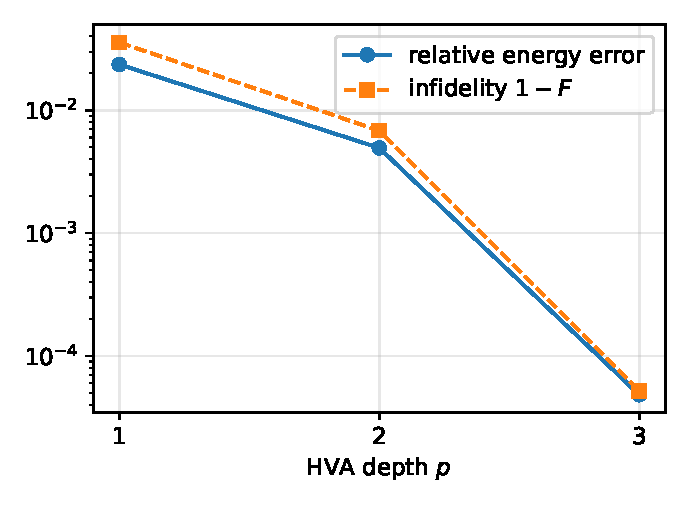
\includegraphics[width=0.62\linewidth]{vqe_depth.pdf}
\caption{Accuracy improves rapidly with HVA depth at the four-site critical point.}
\label{fig:vqe-depth}
\end{figure}

A continuation sweep warm-starts the $p=3$ ansatz from the paramagnetic side toward the ordered regime.  Table~\ref{tab:h-sweep} reports accuracy and physical diagnostics; Fig.~\ref{fig:h-sweep} shows both.  The ansatz remains highly accurate near and above the critical point, while relative error grows in the deeply ordered $h/J=0.2$ regime, where a low-depth symmetric ansatz must approximate a more strongly correlated, nearly degenerate state.

\begin{table}[h]
\centering
\caption{$p=3$ continuation sweep across $h/J$.}
\label{tab:h-sweep}
\begin{tabular}{ccccccc}
\toprule
$h/J$ & $E_{\rm VQE}$ & Rel. error & Fidelity & $\langle X\rangle$ & $\langle ZZ\rangle$ & $S_{1/2}$ \\
\midrule
2.0 & $-8.376790$ & $1.03\times10^{-6}$ & 0.999999 & 0.9525 & 0.2523 & 0.1268 \\
1.4 & $-6.140282$ & $7.88\times10^{-6}$ & 0.999992 & 0.9024 & 0.3623 & 0.2373 \\
1.0 & $-4.758540$ & $4.84\times10^{-5}$ & 0.999948 & 0.8104 & 0.5057 & 0.4190 \\
0.6 & $-3.629601$ & $4.91\times10^{-4}$ & 0.999441 & 0.5623 & 0.7600 & 0.7881 \\
0.2 & $-3.045375$ & $5.34\times10^{-3}$ & 0.992980 & 0.1796 & 0.9672 & 1.0005 \\
\bottomrule
\end{tabular}
\end{table}

\begin{figure}[h]
\centering
\begin{subfigure}{0.48\linewidth}
\centering
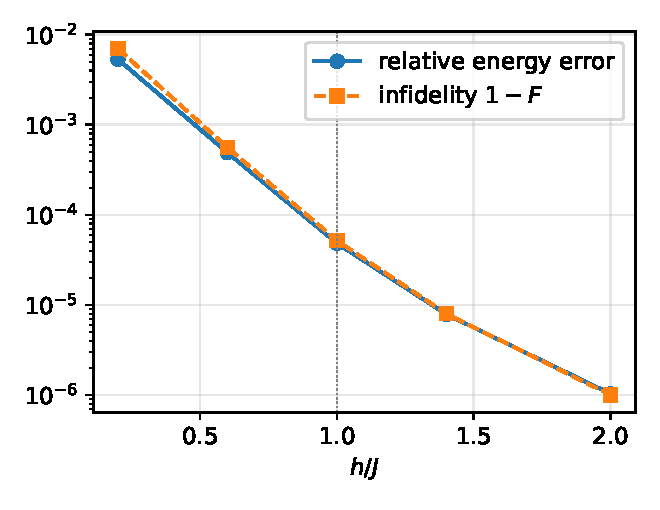
\includegraphics[width=\linewidth]{h_sweep_accuracy.pdf}
\caption{Accuracy and fidelity loss.}
\end{subfigure}
\begin{subfigure}{0.48\linewidth}
\centering
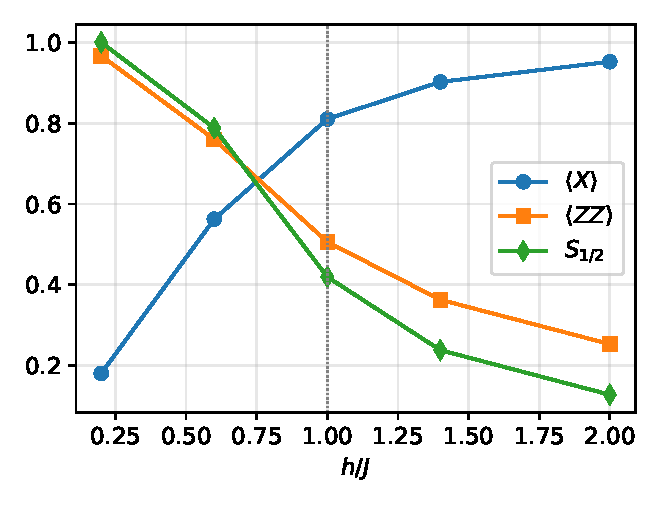
\includegraphics[width=\linewidth]{h_sweep_diagnostics.pdf}
\caption{Order and entanglement diagnostics.}
\end{subfigure}
\caption{Adiabatic continuation with the $p=3$ Pauli-rotation ansatz.}
\label{fig:h-sweep}
\end{figure}

\section{ADAPT-VQE with Finite-Shot Operator Selection}

\subsection{The selection gradient as a Hermitian observable}
\label{sec:selection}

ADAPT-VQE grows the ansatz by selecting the pool operator with the largest energy-gradient magnitude at the current state.  If a candidate generator is $P$, appending $R_P(\theta)$ at $\theta=0$ and applying Eq.~\eqref{eq:rotor-derivative} gives the selection derivative
\begin{equation}
    g_P = \left.\frac{\partial E}{\partial\theta}\right|_{\theta=0}
    =\Tr\left(G_P\rho\right),\qquad
    G_P = -\frac{\ii}{2}[H,P].
    \label{eq:commutator-gradient}
\end{equation}
This is the operator-centric point in miniature: the selection score is not an abstract derivative but the expectation of the Hermitian element $G_P$ of the same algebra, one commutator and one scalar-part read per candidate, with no circuit execution required for ranking.  Since $H$ and $P$ are Hermitian, $G_P$ decomposes into Pauli words with real coefficients,
\begin{equation}
    G_P = \sum_w c_w w,\qquad c_w\in\mathbb{R},
\end{equation}
and on hardware $g_P$ is measured word by word:
\begin{equation}
    \widehat g_P = \sum_w c_w\widehat{\langle w\rangle},
\end{equation}
where each $\widehat{\langle w\rangle}=2k/N-1$ is estimated from $N$ binary outcomes with success probability $(1+\langle w\rangle)/2$.  The oracle variance available in simulation is
\begin{equation}
    \mathrm{Var}(\widehat g_P)=\sum_w c_w^2\frac{1-\langle w\rangle^2}{N},
    \label{eq:oracle-var}
\end{equation}
used only to calibrate the simulator.  Decisions use a hardware-realistic empirical variance with pseudocounts: if $k_w$ successes are observed after $N$ shots for word $w$,
\begin{equation}
    \tilde p_w=\frac{k_w+1/2}{N+1},\qquad
    \tilde m_w=2\tilde p_w-1,\qquad
    \widehat\sigma_{P,\rm emp}^2
    = \sum_w c_w^2\frac{1-\tilde m_w^2}{N+1},
    \label{eq:emp-var}
\end{equation}
which avoids spuriously zero uncertainty when a finite sample happens to return identical outcomes.

\subsection{Local no-repeat pool}

By Proposition~\ref{prop:parity}, only odd-$Y$ words can carry signal, so the pool is a local real-amplitude family centered on $Y_i$ and dressed by neighboring $Z$ factors,
\begin{equation}
    P_{i,S}=\Bigl(\prod_{j\in S}Z_j\Bigr)Y_i,
\end{equation}
where $S$ may contain the immediate left neighbor, the immediate right neighbor, or both, subject to open-chain boundaries.  A periodic-context option exists for controlled ablations, but the default pool avoids wrap-around operators on an open-chain Hamiltonian, matching linear hardware connectivity.  A no-repeat rule prevents selecting the same operator twice; the three-local $ZYZ$ terms supply enough local expressivity to recover the hard low-field case without repeated generators.

\subsection{Cumulative escalation and statistical gates}

The finite-shot loop uses cumulative escalation: if a candidate has already been measured with $N$ shots per word and the target doubles to $2N$, only the extra $N$ shots are added, which is distributionally equivalent to a single larger binomial batch and wastes no measurements.

At each step the algorithm scores all unused candidates and applies two heuristic gates.  These are transparent decision rules, not simultaneous confidence guarantees: the per-word variances are combined assuming independent sampling (Section~\ref{sec:selection}), no multiple-comparison correction is applied across the pool, and the leading score is subject to winner-selection bias.
\begin{enumerate}[leftmargin=*]
    \item \textbf{Nonzero-signal gate.}  The leading score must satisfy
    $|\widehat g_{(1)}| \ge k\,\widehat\sigma_{(1)}$ with $k=3$ by default.  The deterministic convergence threshold $\epsilon$ is applied only \emph{after} this statistical check; using $\epsilon$ itself as a significance test is unsound, since any noise estimate exceeds a small fixed $\epsilon$.
    \item \textbf{Rank-resolution gate.}  When rank resolution is required, the top two candidates must satisfy
    $|\widehat g_{(1)}|-|\widehat g_{(2)}| \ge k\sqrt{\widehat\sigma_{(1)}^2+\widehat\sigma_{(2)}^2}$.
    If exact or symmetry-induced ties prevent resolution even at the shot ceiling, the best statistically nonzero candidate is accepted.
\end{enumerate}
The ablation keeps parameter re-optimization exact, isolating the question of whether adaptive growth survives stochastic \emph{ranking}.  Because each appended gate starts at $\theta=0$ and the previous optimum remains feasible, the optimized energy cannot rise when an operator is added.  This protects the variational bound but does not undo a bad pick: exact re-optimization keeps the energy non-increasing, yet a wasted operator permanently occupies a slot in the ansatz and the shots spent selecting it cannot be reclaimed.

\subsection{Noisy ADAPT results}

Exact selection reaches numerical ground-state accuracy for the four-site critical open chain with six operators.  The finite-shot estimator is empirically calibrated: the estimator mean lies within the expected sampling band and the empirical-to-predicted standard-deviation ratio is $1.017$.

Table~\ref{tab:adapt} summarizes a finite-shot robustness sweep with $30$ seeds at each base budget of $32$, $128$, and $512$ shots per Pauli word, with cumulative escalation by up to $32\times$; Fig.~\ref{fig:adapt} shows the accuracy--cost tradeoff.  We report the fraction of seeds reaching relative energy error below $10^{-3}$ together with the median total measurement cost.  The success rate rises steeply with the base budget while the measurement cost grows roughly linearly, so the base budget buys ranking reliability rather than a lower accuracy floor.

\begin{table}[h]
\centering
\caption{Noisy ADAPT selection robustness at $n=4$, $h/J=1.0$, $30$ seeds per base budget, escalation $\times32$.  Success is relative energy error below $10^{-3}$.}
\label{tab:adapt}
\begin{tabular}{ccc}
\toprule
Base shots per word & Success rate ($<10^{-3}$) & Median total shots \\
\midrule
32  & 20.0\% & $0.168$ million \\
128 & 80.0\% & $0.813$ million \\
512 & 93.3\% & $2.830$ million \\
\bottomrule
\end{tabular}
\end{table}

\begin{figure}[h]
\centering
\begin{subfigure}{0.48\linewidth}
\centering
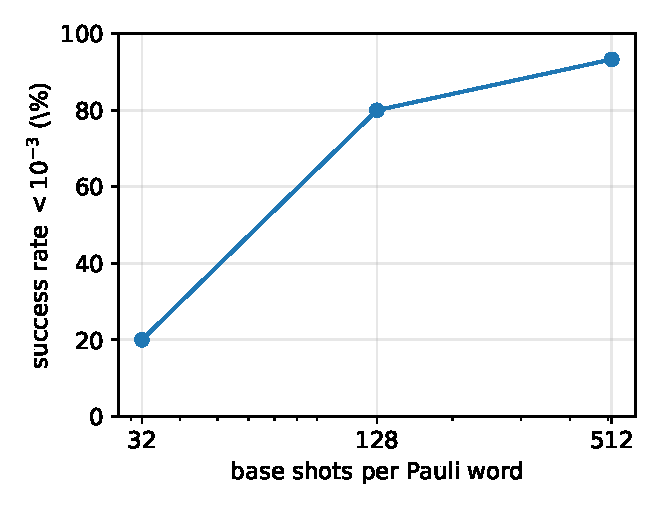
\includegraphics[width=\linewidth]{adapt_robustness.pdf}
\caption{Success rate.}
\end{subfigure}
\begin{subfigure}{0.48\linewidth}
\centering
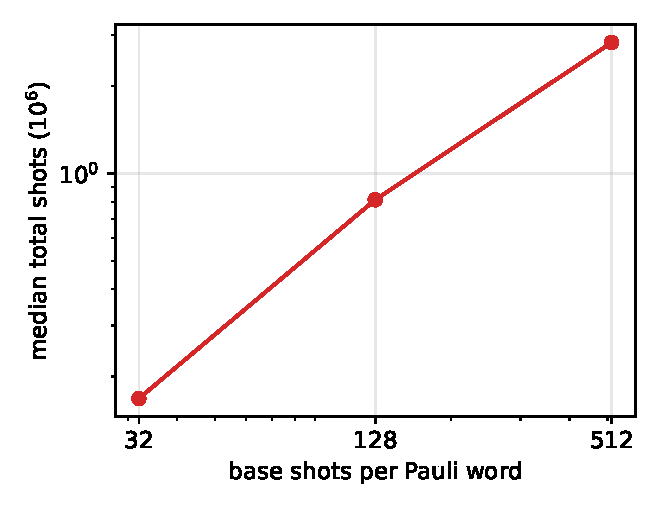
\includegraphics[width=\linewidth]{adapt_shots.pdf}
\caption{Measurement cost.}
\end{subfigure}
\caption{Finite-shot ADAPT selection: success rate and measurement cost as functions of the base shot budget, showing that shots buy ranking reliability.}
\label{fig:adapt}
\end{figure}

A representative low-shot run selected five operators and stopped when no statistically resolvable gradient remained, with final relative error $5.15\times10^{-5}$, fidelity $0.999956$, and total measurement cost $0.20$ million shots.  Every noisy run in the tested sweep preserved purity and the variational lower bound, and the optimized energy was non-increasing as operators were added.

\section{Discussion}

The main conceptual benefit of the operator-centric formulation is the removal of artificial boundaries between objects.  Gates, density operators, observables, channels, fermionic modes, Hamiltonian terms, and selection gradients all live in the same sparse algebra.  Pauli-word rotations are not merely matrix exponentials but closed-form Clifford-algebra elements whose one-line derivative, Eq.~\eqref{eq:rotor-derivative}, yields both the parameter-shift identity and the adjoint gradient.  ADAPT selection gradients are not abstract derivatives but explicit Hermitian observables, decomposed into measurable Pauli words whose statistics obey Eqs.~\eqref{eq:oracle-var}--\eqref{eq:emp-var}.  And the $Y$-parity grading of the word basis turns an operator-pool design heuristic into a short proposition (Proposition~\ref{prop:parity}).

Two methodological cautions emerge from the analysis.  First, parameter-shift identities must be applied to physical gates, not blindly to shared parameters that control several noncommuting gates; the adjoint sweep is the correct exact-gradient tool for shared-parameter ansatzes.  Second, a deterministic convergence threshold such as $\epsilon=10^{-6}$ must never double as a statistical significance test under finite-shot noise: the correct order asks first whether a signal is statistically nonzero, and only then applies $\epsilon$ as a deterministic convergence criterion.  Violating this ordering silently degrades adaptive selection to fixed-shot ranking with premature stopping.

The rank-resolution gate explains the economics of selection.  At symmetric points, exact ties make ranking impossible at any shot count; the algorithm correctly escalates to its ceiling and accepts an ambiguous but statistically nonzero candidate.  Accepting an ambiguous candidate is safe for the variational bound --- subsequent re-optimization keeps the energy non-increasing --- but it is not free: the accepted operator may be a poor choice that consumes an ansatz slot and the shots already spent, and this waste is not recovered later.  Replacing the all-candidates-to-the-same-$N$ policy with successive halving, racing, or bandit-style pruning, so that obvious losers are not remeasured to the ceiling reached by plausible winners, is a natural next step.  Pool locality matters for the same practical reason: a periodic-context pool can be variationally useful for an open-chain Hamiltonian, but it introduces wrap-around operators that are nonlocal on linear hardware; the default pool respects the boundary conditions of the problem.

\section{Limitations}

This work is a classical study and claims no quantum speedup.  Exact diagonalization provides validation targets, and re-optimization is kept exact in the noisy-selection ablation to isolate the effect of stochastic operator ranking.  A physical-device implementation would add optimizer shot noise, hardware decoherence, state-preparation and measurement errors, calibration drift, connectivity constraints, and measurement-grouping overhead.  Several idealizations in the finite-shot model should be made explicit: each Pauli word is sampled independently, so covariance between co-measurable words, commuting-group simultaneous measurement, and shot reuse across candidates are all neglected; the statistical gates are heuristics without a simultaneous-confidence guarantee and the leading score carries winner-selection bias; and the reported per-word shot counts are a simple baseline rather than a measurement-optimal cost, which grouping and classical-shadow techniques would reduce.  The numerical results are for $n=4$; they establish correctness and qualitative behavior rather than scaling performance.  Finally, while Pauli-word sparsity is structurally meaningful for Clifford-like circuits and low-depth Pauli-rotation ansatzes, generic non-Clifford evolution grows the active word support rapidly, and dense methods are then preferable.

\section{Conclusion}

We have presented an operator-centric Clifford-algebra formulation of variational quantum simulation and applied it to the transverse-field Ising chain.  One algebra carries the entire theory: density multivectors, Pauli-word rotation gates, channels, fermionic modes, entanglement operations as coefficient surgery, and adaptive selection gradients as Hermitian commutator observables.  Within this formulation, a Pauli-rotation Hamiltonian variational ansatz achieves high fidelity at small depth; a reality selection rule fixes the ADAPT operator pool a priori; and finite-shot ADAPT with cumulative escalation and heuristic statistical gates remains variational and monotone while making the measurement economics of adaptive selection explicit.  The framework offers a compact, fully reproducible setting in which geometric algebra, variational ansatz design, and measurement-limited adaptive selection can be studied in one computational language.

\section*{Code Availability}

All numerical results, tables, and figures in this paper are reproducible from the open-source repository at
\url{https://github.com/gutama/clifford_qc}.

\appendix

\section{Condensed Verification Log}

\begin{table}[h]
\centering
\caption{Condensed verification outcomes underlying the results.}
\begin{tabular}{p{0.28\linewidth}p{0.62\linewidth}}
\toprule
Layer & Key verified properties \\
\midrule
Algebraic kernel & Associativity, adjoint identity, Clifford anticommutation, inverse Jordan--Wigner decoding, CAR relations, Bell/CHSH/Grover, channel completeness and fixed points, Trotter and exponential dynamics \\
Pauli-rotation VQE & Ansatz unitarity, pure density evolution, Pauli-rotation grade structure, adjoint gradient equals the sum of per-gate parameter shifts and finite differences, single shared-parameter shift detected as non-exact \\
Finite-shot ADAPT & $G_P$ Hermitian with real word coefficients, word-sum equals exact gradient, exact selection reaches numerical ground-state accuracy, estimator unbiased and variance-calibrated, every noisy run pure, variational, and non-increasing in energy \\
\bottomrule
\end{tabular}
\end{table}

\begin{thebibliography}{99}

\bibitem{peruzzo2014vqe}
A. Peruzzo, J. McClean, P. Shadbolt, M.-H. Yung, X.-Q. Zhou, P. J. Love, A. Aspuru-Guzik, and J. L. O'Brien,
``A variational eigenvalue solver on a photonic quantum processor,''
\emph{Nature Communications} \textbf{5}, 4213 (2014).
\url{https://doi.org/10.1038/ncomms5213}

\bibitem{grimsley2019adapt}
H. R. Grimsley, S. E. Economou, E. Barnes, and N. J. Mayhall,
``An adaptive variational algorithm for exact molecular simulations on a quantum computer,''
\emph{Nature Communications} \textbf{10}, 3007 (2019).
\url{https://doi.org/10.1038/s41467-019-10988-2}

\bibitem{tang2021qubitadapt}
H. L. Tang, V. O. Shkolnikov, G. S. Barron, H. R. Grimsley, N. J. Mayhall, E. Barnes, and S. E. Economou,
``Qubit-ADAPT-VQE: An adaptive algorithm for constructing hardware-efficient ansatze on a quantum processor,''
\emph{PRX Quantum} \textbf{2}, 020310 (2021).
\url{https://doi.org/10.1103/PRXQuantum.2.020310}

\bibitem{mitarai2018qcl}
K. Mitarai, M. Negoro, M. Kitagawa, and K. Fujii,
``Quantum circuit learning,''
\emph{Physical Review A} \textbf{98}, 032309 (2018).
\url{https://doi.org/10.1103/PhysRevA.98.032309}

\bibitem{wierichs2022general}
D. Wierichs, J. Izaac, C. Wang, and C. Y.-Y. Lin,
``General parameter-shift rules for quantum gradients,''
\emph{Quantum} \textbf{6}, 677 (2022).
\url{https://doi.org/10.22331/q-2022-03-30-677}

\bibitem{hrdina2022clifford}
J. Hrdina, A. Navrat, and P. Vasik,
``Quantum computing based on complex Clifford algebras,''
\emph{Quantum Information Processing} \textbf{21}, 310 (2022).
\url{https://arxiv.org/abs/2201.02246}
% Spinor / minimal-left-ideal Clifford construction (antecedent to the operator-centric picture).

\bibitem{silva2025operator}
% TODO: verify exact title, venue, and arXiv identifier from the project references before submission.
A. Silva,
``Operator-centric quantum computation in complex Clifford algebra,''
preprint (2025).

\bibitem{hestenes2003oersted}
D. Hestenes,
``Oersted Medal Lecture 2002: Reforming the mathematical language of physics,''
\emph{American Journal of Physics} \textbf{71}, 104--121 (2003).
\url{https://doi.org/10.1119/1.1522700}

\bibitem{jordan1928}
P. Jordan and E. Wigner,
``\"Uber das Paulische \"Aquivalenzverbot,''
\emph{Zeitschrift f\"ur Physik} \textbf{47}, 631--651 (1928).
\url{https://doi.org/10.1007/BF01331938}

\bibitem{pfeuty1970ising}
P. Pfeuty,
``The one-dimensional Ising model with a transverse field,''
\emph{Annals of Physics} \textbf{57}, 79--90 (1970).
\url{https://doi.org/10.1016/0003-4916(70)90270-8}

\bibitem{aaronson2004stabilizer}
S. Aaronson and D. Gottesman,
``Improved simulation of stabilizer circuits,''
\emph{Physical Review A} \textbf{70}, 052328 (2004).
\url{https://arxiv.org/abs/quant-ph/0406196}

\end{thebibliography}

\end{document}
